\documentclass{report}
\usepackage{graphicx}
\usepackage{subfig}
\usepackage{csquotes}
\usepackage[hidelinks]{hyperref}
\usepackage{mdwlist}
\usepackage[titletoc]{appendix}
\usepackage[backend=biber,sorting=none]{biblatex}
%\addbibresource{references.bib}
\usepackage{fancyhdr}
%glossaries
\usepackage[acronym,shortcuts,nopostdot,style=super,nonumberlist,toc]{glossaries}
\usepackage{glossaries-extra}
%textbox
\usepackage{tcolorbox}
%encoding
\usepackage[utf8]{inputenc}
\usepackage[T1]{fontenc}
%Portuguese-specific commands
\usepackage[portuguese]{babel}
%Hyphenation rules
\usepackage{hyphenat}
\hyphenation{mate-mática recu-perar}
\usepackage{everypage}
%
\usepackage{xstring}
\usepackage{listings}


\makeatletter
\renewcommand
   {\appendixtocname}{Ap\^{e}ndices}
 \renewcommand
   {\appendixpagename}{Ap\^{e}ndices}
 \renewcommand
   {\appendixname}{Ap\^{e}ndice} \let\oriAlph\Alph
 \let\orialph\alph
 \renewcommand{\@resets@pp}
   {\par\@ppsavesec
     \stepcounter{@pps}%
     \setcounter{section}{0}%
     \if@chapter@pp
       \setcounter{chapter}{0}%
       \renewcommand\@chapapp{\appendixname}%
       \renewcommand\thechapter{\@Alph\c@chapter}%
     \else
       \setcounter{subsection}{0}%
       \renewcommand\thesection{\@Alph\c@section}%
     \fi
     \if@pphyper
       \if@chapter@pp
         \renewcommand
           {\theHchapter}
           {\theH@pps.\oriAlph{chapter}}%
       \else
         \renewcommand
           {\theHsection}
           {\theH@pps.\oriAlph{section}}%
       \fi
       \def\Hy@chapapp
          {appendix}%
     \fi
   \restoreapp
  }
\makeatother





\makeatletter
\renewcommand{\@chapapp}{}% Not necessary...
\newenvironment{chapquote}[2][2em]
  {\setlength{\@tempdima}{#1}%
   \def\chapquote@author{#2}%
   \parshape 1 \@tempdima \dimexpr\textwidth-2\@tempdima\relax%
   \itshape}
  {\par\normalfont\hfill--\ \chapquote@author\hspace*{\@tempdima}\par\bigskip}
\makeatother



\pagestyle{fancy}
\fancyhf{}
\fancyhead[LE,RO]{\leftmark}
\fancyfoot[LE,RO]{\thepage}
\renewcommand{\headrulewidth}{0.2pt}
\renewcommand{\footrulewidth}{0pt}


\bibliography{Chapter/references}


\begin{document}

\begin{titlepage}
\vspace*{\fill}
\begin{center}
{\fontsize{50}{60}\selectfont My IT Recipes}\\[0.5cm]
\begin{figure}[h]
\begin{center}
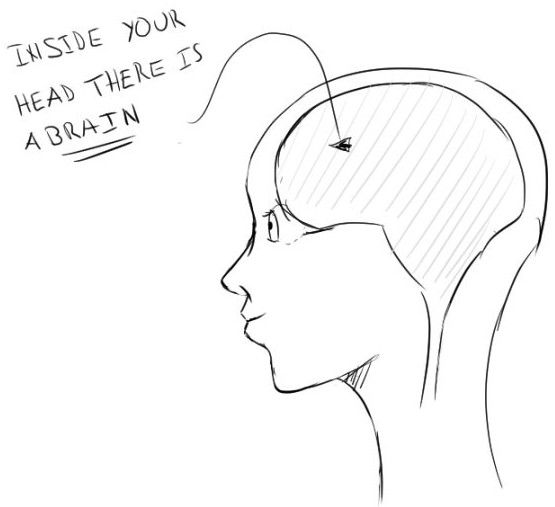
\includegraphics[scale=0.5]{Figs/brain.jpg}
\end{center}
\end{figure}
\vspace{4em}
\textsc{\Large Bernardo Vieira}\\[1em]
\end{center}
\vspace*{\fill}
\end{titlepage}


\begin{abstract}
Thanks to the people I haven't thanked yet.
\end{abstract}
\clearpage
\tableofcontents
\clearpage

\chapter{Introduction}
Lately I will introduce myself.

\chapter{games}
\section{unity3d}


\chapter{communication}
\section{api}
\section{json}

\chapter{storage}
\section{sql}
\subsection{mysql}
\subsection{postgres}

\section{nosql}
\subsection{mongo}
\subsection{neo4j}

\chapter{programming languages}
\section{java}
\subsection{inject parametres on command line}

\section{c}
\subsection{circular dependency}

\section{assembly}
\subsection{registry (and everything else)}


\chapter{frameworks}
\section{nodejs}
\section{rails}

\chapter{vitualization}
\section{virtualbox}
\section{docker}
\subsection{Copy volumes from older containers}
\begin{displayquote}
\$ docker stop my-container \newline
\$ docker rename my-container my-old-container \newline
\$ docker run --volumes-from=my-old-container --restart always myimage \newline
\$ docker rm my-old-container
\end{displayquote}
\subsection{Volumes to a specific folder}
\begin{displayquote}
\$ docker run -v path/at/host:path/inside/container/folder my-image \newline
\end{displayquote}
\subsection{Look for volumes}
\begin{displayquote}
\$ docker inspect my-image \newline
\end{displayquote}
\lstinputlisting[language=Bash]{Chapters/docker_volume_mount.sh}

\chapter{cloud}
\section{azure}

\chapter{ci/cd}
\section{jenkins}
\section{travis}
\section{travis}

\chapter{linux}
\section{commands}
for files in `ls *.tex`; do mv \$files `echo \$files | sed s/oldname/newname/g`; done
\section{bash}
\begin{lstlisting}[language=sh]
#!/bin/bash

echo $1
\end{lstlisting}

\chapter{electronics}
\section{components}
\section{arduino}
\subsection{board}
\subsection{shields}

\chapter{text processors}
\section{LaTeX}

\subsection{Write code in Latex}

\begin{lstlisting}[language=TeX]
\*begin{lstlisting}[language=TeX]
\documentclass{article}
\begin{document}
    Hello World
\end{document}
\*end{lstlisting}
\end{lstlisting}


\subsection{No new page when new chapter begins}
\begin{lstlisting}[language=TeX]
\usepackage{etoolbox}
\makeatletter
\patchcmd{\chapter}{\if@openright\cleardoublepage\else\clearpage\fi}{}{}{}
\makeatother
\end{lstlisting}

\section{markdown}

\section{keys}
\subsection{ssh}
\subsection{gpg}

\chapter{Authentication}
\section{oauth}
\begin{chapquote}{Wikipédia, \textit{https://en.wikipedia.org/wiki/OAuth}}
OAuth is an open standard for access delegation, commonly used as a way for Internet users to grant websites or applications access to their information on other websites but without giving them the passwords.
\end{chapquote}
\subsection{Simple}
% TODO stuff
\subsection{MFA}
\begin{chapquote}{Wikipédia, \textit{https://en.wikipedia.org/wiki/Multi-factor\_authentication}}
Multi-factor authentication (MFA) is a method of computer access control in which a user is granted access only after successfully presenting several separate pieces of evidence to an authentication mechanism – typically at least two of the following categories: knowledge (something they know), possession (something they have), and inherence (something they are).
\end{chapquote}
\subsection{2FA}
\begin{chapquote}{Wikipédia, \textit{https://en.wikipedia.org/wiki/Multi-factor\_authentication}}
Two-factor authentication (also known as 2FA) is a method of confirming a user's claimed identity by utilizing a combination of two different components. Two-factor authentication is a type of multi-factor authentication.
\end{chapquote}
It's really common to see this kind of authentication nowadays. But how this works and how can we create an app that connects to a social network where we have \textit{2FA} activated. Let's see how I've done this.\newline
% TODO stuff

\chapter{version control}
\begin{chapquote}{Wikipédia, \textit{https://en.wikipedia.org/wiki/Version\_control}}
A component of software configuration management, version control, also known as revision control or source control, is the management of changes to documents, computer programs, large web sites, and other collections of information.
\end{chapquote}
\section{git}
\begin{chapquote}{Wikipédia, \textit{https://en.wikipedia.org/wiki/Git}}
Git is a version control system (VCS) for tracking changes in computer files and coordinating work on those files among multiple people. It is primarily used for software development, but it can be used to keep track of changes in any set of files. As a distributed revision control system it is aimed at speed, data integrity, and support for distributed, non-linear workflows.
\end{chapquote}
\subsection{Basic usage}
% TODO stuff

\subsection{Branches}
% TODO stuff

\subsection{Rebase from another master}
Sometimes our project is a fork of another project. It's really common to happen, especially on GitHub where there is a lot of people forking others projects.\newline
But then, there is a problem, if you cant control de remote repository in your account like it's in your computer, how do you update it? It's easy:
\begin{lstlisting}[language=Bash]
$ git remote add other <url>
$ git fetch other
$ git rebase other/master master
$ git push
\end{lstlisting}

\chapter{The End}
It's been a pleasure.

\end{document}


\end{document}
